

%%--F1
\begin{figure}[h]
  \centering
  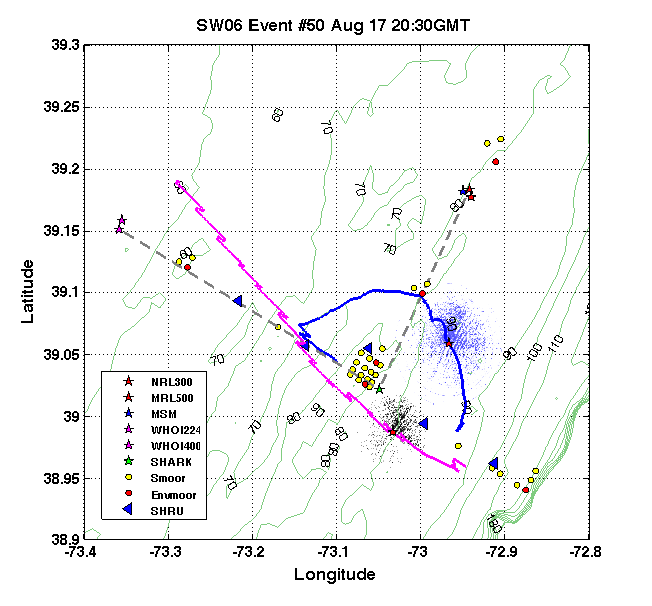
\includegraphics[width=\textwidth]{Aug17_2030_t.png}
  \caption{Surface expression of internal wave package at 20:30GMT, Aug. 17, recorded by R/V Sharp and R/V Oceanus. Blue and red lines indicate their movements, respectively. (Blue: R/V Sharp's, red: R/V Oceanus'}\label{fig:r2130_r}
\end{figure}

\begin{figure}[h]
  \centering
  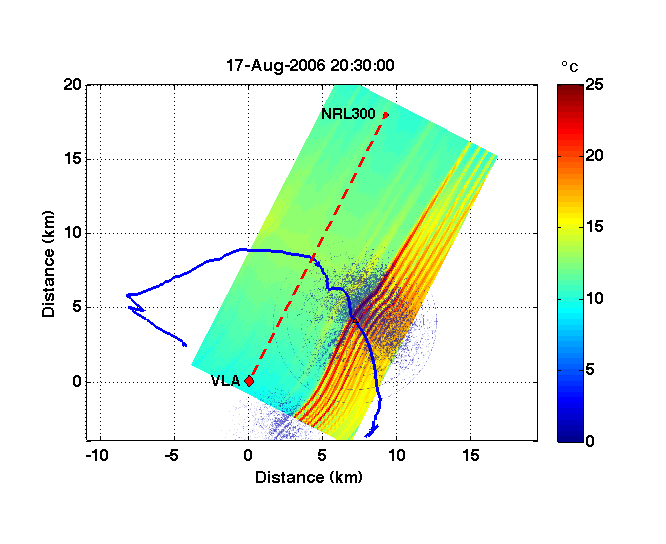
\includegraphics[width=\textwidth]{sw06_Tempr_Depth30m_2006Aug17_203000_radar_curve_thesis1.png}
  \caption{Interpolated internal wave field at 21:30GMT, Aug. 17, water depth = 20m. (Refer to section 3.4 for detailed interpolation method)}\label{fig:r2130_i}
\end{figure}

\begin{figure}[h]
  \centering
  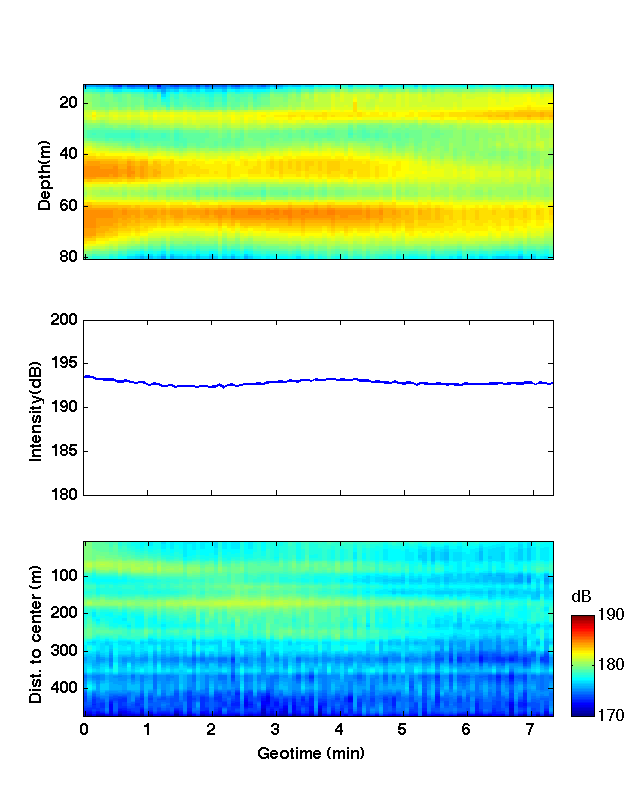
\includegraphics[width=\textwidth]{nrl300_060817T2030_vla_hla_intens_geotime2.png}
  \caption{Received signal on Shark VLA (top), HLA (bottom) and signal intensity (middle) from Aug.17 21:30GMT to 21:37GMT }\label{fig:a2130}
\end{figure}

\begin{figure}[h]
  \centering
  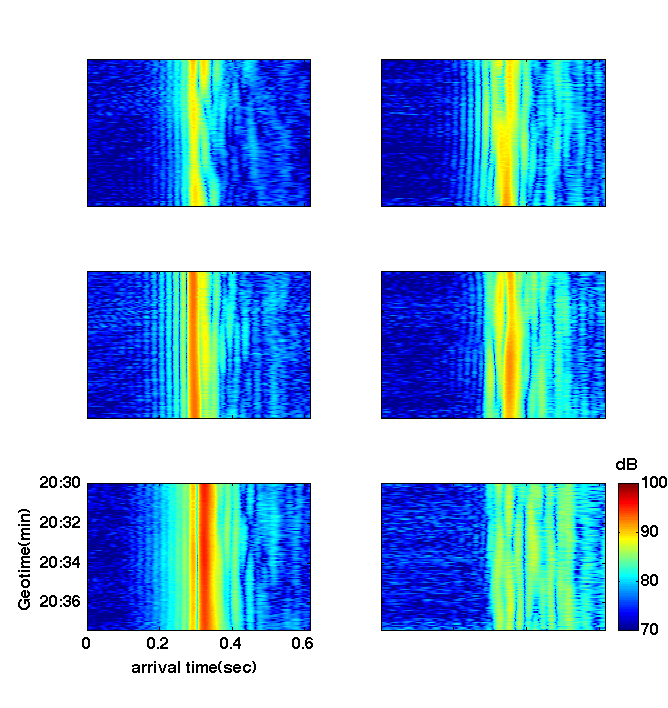
\includegraphics[width=\textwidth]{sw06_broadband_mf_nrl300_F1_6in1_thesis.png}
  \caption{Mode decomposition of received signal on Shark VLA. 
    Left column: mode 1-3, right column: mode 4-6 }\label{fig:m2130}
\end{figure}

